\documentclass[12pt,letterpaper]{article}
\usepackage{amsmath,amsthm,amsfonts,amssymb,amscd}
\usepackage{booktabs}
\usepackage{fullpage}
\usepackage{lastpage}
\usepackage{enumerate}
% \usepackage[nofiglist, notablist]{endfloat}
\usepackage{fancyhdr}
\usepackage{hyperref}
\usepackage{mathrsfs}
\usepackage{natbib}
\usepackage{xcolor}
\usepackage{setspace}
\usepackage{tikz}
% \usepackage{times}
\usetikzlibrary{arrows}
\usetikzlibrary{matrix}
\usepackage[margin=3cm]{geometry}
\setlength{\parindent}{0.25in}
\setlength{\parskip}{0.05in}

\usepackage{compsci430}

\setlength{\parindent}{0.5in}


\newenvironment{answer}[1]{
  \subsubsection*{Question #1}
}


\long\def\cps590header{\begin{center}
\large\bf CPS 430/590.06 \hfill Prof.\ John Reif\\
\large\bf Design and Analysis of Algorithms \hfill Fall 2013 \\
\large\bf Final Project \hfill Matt Dickenson
\end{center}}

\headsep 10pt

\begin{document}

\cps590header

\vspace{1in}
\begin{center}
\textbf{Machine Learning Algorithms with Application to Political Event Data}
\end{center}

\vspace{1in}
\paragraph{Abstract} How do computational and statistical efficiency interact, and what are the trade-offs between them? In the era of ``big data'' this question has become increasingly relevant. This project explores that question in the context of a particular machine learning algorithm (classification trees) and a particular problem (automated processing of political indicators). Applying machine learning to the classification of political event data can greatly reduce the cost in human effort, time, and money. The motivation for this project is to update the Militarized Interstate Disputes (MID) dataset, which has been widely used in academic research and policy discussions. The MID project relies on humans reading journalistic accounts and manually entering the classification of the event according to a defined schema. This dependence on humans is less accurate, less efficient, and more expensive than automated methods. The results of this analysis suggest that automated methods can provide a first-pass classification of political indicators at a huge savings of time and money, without sacrificing interpretability. 


\pagebreak
\doublespacing

\section{Introduction} % introduce the problem and the algorithm

Can computational methods detect political and social upheaval through automated text processing and machine learning? If so, can this process be done with both statistical and computational efficiency? This project seeks to answer these questions in one particular application area: international conflicts. In this section, we provide context for the relevance of this application and the methods under discussion. Section \ref{lit} discusses existing methods for predicting disputes, surveys the extent of machine learning within political science, and explains why classification trees are an appropriate method for this problem. Section \ref{complexity} analyzes the computational complexity of classification trees in general, and Section \ref{analysis} describes the implementation of classification trees used in this project. Section \ref{results} presents the statistical results and compares their efficiency to generalized linear models. Section \ref{conclusion} concludes the paper with implications for future research. 

\section{Background and Motivation} % lit review
\label{lit}

\subsection{Production of MID Data}

The current production of the Militarized Interstate Disputes (MID) dataset is overseen by the Correlates of War Project, headquartered at Penn State University. The most recent version of the data set, MID 3.0, was released in 2003 with coverage through 2001. An update was expected during the summer of 2012, but has been delayed indefinitely. The time-intensive nature of the current MIDS production pipeline inevitably delays important scholarly research on the nature of interstate conflict. 

A ``militarized incident is defined as a single military action involving an explicit threat, display, or use of force by one system member state towards another system member state.'' These incidents form the basis of a dispute in the data set. The current ``algorithm'' for producing MID data updates is as follows \citep{ghosn2004mid3}:

\begin{enumerate}
\item Search the Lexis-Nexis database for news articles mentioning possible militarized incidents. An event classifies as a militarized interstate incident if it:
	\begin{itemize}
		\item occurs among two or more interstate system members;
		\item is an overt action taken by the official military forces or government representatives of a state; and
		\item involves the threat, display, or use of forces.
	\end{itemize}
\item Human coders assigned to a specific geographical region read news articles and list all possible militarized incidents.
\item Principal invesigators classify incidents as ``OK'' or ``under revision.'' More precise information (e.g. exact start date of a conflict) is sought for incidents in the latter category.
\item Events from different regions are aggregated into the final dataset. 
\end{enumerate}

For the most recent update, this process took about three years. By contrast, a single run of a classification tree like the one used in the paper takes less than ten minutes. 

% decision trees can imitate the human thought process while maintaining interpretability 
Decision trees can help to imitate this human thought process, but with obvious advantages in scale and speed \citep{king2003automated, mikhaylov2012coder, ruggeri2011events}. Furthermore, automated methods follow their decision rules perfectly, without falling prey to accidental errors of human classifiers. These trees also maintain interpretability relative to other ``black-box'' machine learning methods, meaning that a well-defined tree could be incorporated into a production pipeline that also includes human classifiers. For all of these reasons, classification trees are worth exploring in this project. 

\subsection{Previous Research}

As one of the most widely used dependent variables in international conflict studies, much effort has been devoted to estimating models of MID onset and duration. However, this work suffers from several common weaknesses that this project attempts to ameliorate: virtually all projects, especially before the present decade, used a fixed functional form (typically from the family of generalized linear models); out-of-sample testing and cross-validation is used only rarely, making claims of `prediction' somewhat dubious in many cases; and often the independent variables are measured at the annual level with high levels of serial correlation, meaning that there is little temporal variation in the predictors, while the dependent variable tends to exhibit more sudden onsets \citep{ward2010perils}. A recent shift toward event data has helped to address the latter two of these issues: with frequent updates (often measured at the daily level), there is substantial variation in the independent variables, validation requires only a brief waiting period for new sets of test data \citep{gerner1994,gerner:etal:2002,king2003automated,ruggeri2011events,schrodt2013gdelt}. 

With this transition toward event data as predictors, the political forecasting community has become attune to new challenges and has responded with several established practices. Coding the sentiment of interactions can now be done in near real-time (NRT) using the Tabari system, which aggregates and deduplicates news reports \citep{o2010crisis,schrodt2009tabari}. Sentiment coding can be done according to two widely used systems. The Goldstein scale assigns a score of -10 (highly conflictual) to +10 (highly cooperative) to events, but it is difficult to employ this scale for aggregations or permutations of the data \citep{goldstein1992conflict}. CAMEO classifies events into a pre-defined schema of material/verbal and cooperative/conflictual actions, that makes aggregation simpler because we can count events within each category \citep{gerner:etal:2002}. These event classifications provide a principled, automated method for exhaustively categorizing  the types of events that may consitute an interstate dispute \citep{ghosn2004mid3}.

The community has also dealt with challenges when aggregating event data up to various temporal levels. Although there is no single best practice, monthly aggregation has become a common strategy \citep{arva2013improving,yonamine2013event} and is used in this project. Modfiying the features by transforming the raw counts into month-to-month changes (i.e. first-differencing) and measuring the balance between conflictual and cooperative interactions as a percentage of the total also helped to simplify the feature set \citep{Box:1976}. 

Interpretability is an important concern in this project due to the policy-relevant nature of the problem and the (potential) need to compare the resulting model to the process used by human coders involved in creating the MID dataset \citep{ghosn2004mid3}. For this reason, ``black box'' methods such as Support Vector Machines were judged to be inappropriate. Classification trees (and their continuous counterpart, regression trees, collectively known as CART) offer a nice alternative that is more flexible than GLMs and more interpretable than Random Forests (these two methods should provide lower and upper bounds, respectively, on CART) \citep{klebanov2008lexical}. CART has been used for event data within conflict studies, and in public health where researchers encounter similar issues of unbalanced and missing data \citep{schrodt1990predicting,speybroeck2012classification,trappl1996digging}.

In later stages of this project, several additional tools may help to improve the predictive accuracy of the model. International conflict is a relatively rare event, meaning that in $k$-fold cross validation it is possible that some subsets will have no instances of conflict; to prevent this, synthetic minority over-sampling (SMOTE) could be used \citep{chawla2002smote}. To incorporate interdependencies not captured at the dyadic level, future iterations could also include lags that measure conflict in social or spatial neighbors \citep{gleditsch2000war,gleditsch2001measuring,hoff2004modeling,ward1998democratizing,ward2007disputes,ward2011network}. A Bayesian ensemble model of several classification trees could also improve performance while still maintaining more interpretability than is available in random forests \citep{arva2013improving,montgomery2012improving,Raftery:1995,raftery2005using}. If these methods are successful, the general processing of automating political indicators through the use of event data could also be applied to other widely used indices such as the Polity and Freedom House regime scales (measuring democracy and autocracy). 


\section{Computational Complexity of Classification Trees}
\label{complexity}

A classification tree provides a set of decision nodes used to assign observations to one or more categories based on features of the observation. We wish to build a tree that minimizes classification error. The problem of finding the optimal tree is NP-complete \citep{mohri2012foundations}. However, we can use a greedy algorithm to grow the tree iteratively, starting at the root. 

A schematic tree consists of a node that \emph{splits} the data based on a \emph{test}. Values satisfying the test are classified into the left subtree, while values failing the test are assigned to the right subtree. Once an observation reaches a leaf node, it is classified probabilistically based on the preponderance of observations assigned to that leaf. 

\begin{figure}
  \begin{center}
    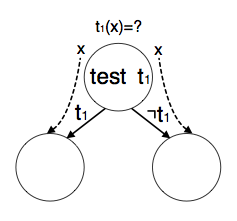
\includegraphics{../graphics/tree-schematic.png}
    \caption{A Schematic of a Classification Tree (adapted from Latkowski, 2003)}
    \label{tree}
  \end{center}
\end{figure}

CART greedily grows a tree $T$ from a root node by adding splits based on features. At each stage, there is an impurity function $I(T)$ that measures the (in)accuracy of the existing classifications. When adding another split to the tree, the CART algorithm seeks to maximize the impurity reduction $\Delta I$. The measure of impurity reduction is supplied to the algorithm, as is a complexity parameter, $\kappa$. We can think of $\kappa$ as the cost of adding another variable to the tree. When $\kappa=\infty$ the tree will consist of only the root node, and as we reduce $\kappa$ toward zero we allow the tree to grow. However, setting $\kappa$ too low can result in overfitting, which can be assessed via cross-validation. For more on classification trees in general and the implementation used for this project, see \citep{murphy2012machine,olshen1984classification,therneau1997introduction}. For $n$ observations, classification is at least as complex as sorting, giving us a lower bound of $\Omega(n \log n)$. Careful implementation with greedy algorithms can reach $\Theta(n \log n)$ \citep{latkowski2003high}. 

Given a set of features $H$, a cost function $I(T)$, and a minimum complexity $\kappa$, the greedy top-down tree-building algorithm at is as follows:

\begin{enumerate}
  \item Initialize the empty tree, $T_0$
  \item Until $\Delta I \leq kappa$:
  \begin{enumerate}
  	\item Given $T_{i-1}$, choose the leaf $l$ and feature test $h \in H$ that maximizes $\Delta I$
  	\item Replace leaf $l$ in $T_i$ with the new subtree created by test $h$
  \end{enumerate}
\end{enumerate}

Pruning is a bottom up procedure that replaces nodes with leaves, minimizes the error in another data set (not the one used to train the tree). This second data set can be an entirely new test set or a bootstrapped version of the original training set. Pruning is generally exponential, but this can be reduced using dyanmic programming. Starting with the errors at each leave, we prune backwards until we reach a threshold (provided as input) for the maximum number of errors, $e$. This gives us the simplest tree possible that makes no more than $e$ errors. For data input of size $n$ and tree size $|T|$, greedy pruning can be done in $O(n^2 |T|)$. Having seen how classification trees perform in theory and their computational efficiency, we now turn to an applied case to examine their statistical efficiency and accuracy.


\section{Applied Analyis}
\label{analysis}

\subsection{Problem Definition and Data Sources}

The classification tree attempts to categorize country dyad months (e.g. \texttt{USA-China-2012-May}) as either in conflict or not. To achieve this, we use real time (daily) event data from the Global Database of Events, Language, and Tone (GDELT), aggregated up to the dyad month level for 1992-present \citep{schrodt2013gdelt}. To measure the dependent variable of conflict, the Militarized Interstate Disputes (MID) dataset will be split into subsets for training and validation \citep{ghosn2004mid3}. The goal of this project is to replicate and extend MID data coding as accurately as possible using automated procedures. If a reliable method can be developed to replicate the MID data up to 2001, it can then be extended to generate data for interstate disputes since 2001. 

In work on this project thus far, several important features of the GDELT data have been identified. All events in GDELT are classified according to the CAMEO coding scheme \citep{gerner:etal:2002}. Within this scheme, there are two major distinctions along two dimensions: acts can be material or verbal, and interactions can be cooperative or conflictual. These four categories provide a rough characterization of how two countries interact within a given period of time. More fine-grain classification, into twenty subcategories, is also provided. Verbal cooperative events include public statements, appeals, expressions of intent to cooperate, consultations, and engaging in diplomatic cooperation. Materiale cooperation includes providing aid, yielding, and investigations. Verbal conflict includes demands, disapproval, rejections of offers, threats, and protests. Material conflict includes exhibiting force posture, reducing relations, coercion, assaults, fights, and the use of unconventional mass violence. These categories are mutually exclusive and exhaustive. 

During the process of aggregating GDELT records into dyad months, the absolute number of events within each of the four major and twenty minor categories was counted. From these raw counts, the monthly change in counts and percentages, as well as the relative frequency of each interaction type was computed. These features--proportion of interactions that were conflictual versus cooperative, and how sharply events changed from the previous month--will be used as predictors for the classification procedure. 

MID hostilities are measured on a five-point scale, which was collapsed into a binary with the cutoff set at four. Events above this threshold involve the use of force, typically associated with ``war,'' while events below this threshold require only the threat or display of force \citep{ghosn2004mid3}. Further classification of exact hostility levels will be attempted in a later stage of this project. 

\subsection{Model}

The conflict indicators $y_{i,j,t}$ are binary $(0,1)$. The observations $x_{i,j,t}$ consist of the month-to-month change in interactions between $i$ and $j$ within each of the event categories described above ($\Delta x_{i,j,t} = x_{i,j,t} - x_{i,j,t-1}$). Thus, $x$ is a count variable that can take on positive or negative values ($x \in \mathbb{Z}$). The observations $z_{i,j,t}$ measure the relative frequency of conflictual interactions as a percentage of the total $n$ observations for the dyad-month: 

The predictor values are observed in the GDELT data. The indicator of conflict, $y$, is observed in the MID data, and predicted indicators of conflict $\hat{y}$ will be estimated. The predicted values $\hat{y}$ for the test set can be compared to the actual MID data to assess how well the model works out-of-sample. This will give us a sense of how accurate the classifications for post-2001 data will be. Even though these values will not be perfectly accurate, they should give us a good approximation of which countries experienced conflict since 2001 and can help speed up the production of the next generation of MID data. A classification tree was fit to this data, with results presented in the next section.


\section{Results}
\label{results}

To fit the classification tree, this project used the \texttt{rpart} library in $\mathcal{R}$ \citep{therneau1997introduction}. The minimum complexity parameter, $\kappa$, was initialized to be $10^{-4}$. By cross-validation, the optimal $\kappa$ was found to be 0.00155 (see Figure \ref{cpplot}). This value was used to prune the tree from its maximum of 176 splits down to nine. The resulting tree is shown in Figure \ref{tree}, with leaves shaded by whether MID hostilities (``war'') or peace is more likely. Each leaf also indicates the relative frequency of war in the training set for observations assigned to that leaf.

\begin{figure}
  \begin{center}
    % Created by tikzDevice version 0.6.4 on 2013-12-03 10:14:35
% !TEX encoding = UTF-8 Unicode
\begin{tikzpicture}[x=1pt,y=1pt]
\definecolor[named]{fillColor}{rgb}{1.00,1.00,1.00}
\path[use as bounding box,fill=fillColor,fill opacity=0.00] (0,0) rectangle (433.62,361.35);
\begin{scope}
\path[clip] ( 49.20, 61.20) rectangle (408.42,312.15);
\definecolor[named]{drawColor}{rgb}{0.00,0.00,0.00}

\path[draw=drawColor,line width= 0.4pt,line join=round,line cap=round] ( 62.50,152.77) --
	( 77.62,153.50) --
	( 92.74,152.03) --
	(107.86,152.03) --
	(122.98,155.96) --
	(138.10,156.95) --
	(153.22,158.43) --
	(168.34,158.43) --
	(183.45,161.38) --
	(198.57,161.87) --
	(213.69,162.61) --
	(228.81,170.49) --
	(243.93,170.49) --
	(259.05,175.90) --
	(274.17,186.24) --
	(289.28,190.67) --
	(304.40,199.77) --
	(319.52,203.71) --
	(334.64,204.21) --
	(349.76,212.57) --
	(364.88,214.30) --
	(380.00,220.70) --
	(395.12,220.70);

\path[draw=drawColor,line width= 0.4pt,line join=round,line cap=round] ( 62.50,152.77) circle (  2.25);

\path[draw=drawColor,line width= 0.4pt,line join=round,line cap=round] ( 77.62,153.50) circle (  2.25);

\path[draw=drawColor,line width= 0.4pt,line join=round,line cap=round] ( 92.74,152.03) circle (  2.25);

\path[draw=drawColor,line width= 0.4pt,line join=round,line cap=round] (107.86,152.03) circle (  2.25);

\path[draw=drawColor,line width= 0.4pt,line join=round,line cap=round] (122.98,155.96) circle (  2.25);

\path[draw=drawColor,line width= 0.4pt,line join=round,line cap=round] (138.10,156.95) circle (  2.25);

\path[draw=drawColor,line width= 0.4pt,line join=round,line cap=round] (153.22,158.43) circle (  2.25);

\path[draw=drawColor,line width= 0.4pt,line join=round,line cap=round] (168.34,158.43) circle (  2.25);

\path[draw=drawColor,line width= 0.4pt,line join=round,line cap=round] (183.45,161.38) circle (  2.25);

\path[draw=drawColor,line width= 0.4pt,line join=round,line cap=round] (198.57,161.87) circle (  2.25);

\path[draw=drawColor,line width= 0.4pt,line join=round,line cap=round] (213.69,162.61) circle (  2.25);

\path[draw=drawColor,line width= 0.4pt,line join=round,line cap=round] (228.81,170.49) circle (  2.25);

\path[draw=drawColor,line width= 0.4pt,line join=round,line cap=round] (243.93,170.49) circle (  2.25);

\path[draw=drawColor,line width= 0.4pt,line join=round,line cap=round] (259.05,175.90) circle (  2.25);

\path[draw=drawColor,line width= 0.4pt,line join=round,line cap=round] (274.17,186.24) circle (  2.25);

\path[draw=drawColor,line width= 0.4pt,line join=round,line cap=round] (289.28,190.67) circle (  2.25);

\path[draw=drawColor,line width= 0.4pt,line join=round,line cap=round] (304.40,199.77) circle (  2.25);

\path[draw=drawColor,line width= 0.4pt,line join=round,line cap=round] (319.52,203.71) circle (  2.25);

\path[draw=drawColor,line width= 0.4pt,line join=round,line cap=round] (334.64,204.21) circle (  2.25);

\path[draw=drawColor,line width= 0.4pt,line join=round,line cap=round] (349.76,212.57) circle (  2.25);

\path[draw=drawColor,line width= 0.4pt,line join=round,line cap=round] (364.88,214.30) circle (  2.25);

\path[draw=drawColor,line width= 0.4pt,line join=round,line cap=round] (380.00,220.70) circle (  2.25);

\path[draw=drawColor,line width= 0.4pt,line join=round,line cap=round] (395.12,220.70) circle (  2.25);
\end{scope}
\begin{scope}
\path[clip] (  0.00,  0.00) rectangle (433.62,361.35);
\definecolor[named]{drawColor}{rgb}{0.00,0.00,0.00}

\node[text=drawColor,anchor=base,inner sep=0pt, outer sep=0pt, scale=  1.00] at (228.81, 15.60) {$\kappa$};

\node[text=drawColor,rotate= 90.00,anchor=base,inner sep=0pt, outer sep=0pt, scale=  1.00] at ( 10.80,186.67) {Cross-Validated Relative Error};
\end{scope}
\begin{scope}
\path[clip] (  0.00,  0.00) rectangle (433.62,361.35);
\definecolor[named]{drawColor}{rgb}{0.00,0.00,0.00}

\path[draw=drawColor,line width= 0.4pt,line join=round,line cap=round] ( 49.20, 61.20) --
	(408.42, 61.20) --
	(408.42,312.15) --
	( 49.20,312.15) --
	( 49.20, 61.20);

\path[draw=drawColor,line width= 0.4pt,line join=round,line cap=round] ( 49.20, 84.17) -- ( 49.20,289.95);

\path[draw=drawColor,line width= 0.4pt,line join=round,line cap=round] ( 49.20, 84.17) -- ( 43.20, 84.17);

\path[draw=drawColor,line width= 0.4pt,line join=round,line cap=round] ( 49.20,118.47) -- ( 43.20,118.47);

\path[draw=drawColor,line width= 0.4pt,line join=round,line cap=round] ( 49.20,152.77) -- ( 43.20,152.77);

\path[draw=drawColor,line width= 0.4pt,line join=round,line cap=round] ( 49.20,187.06) -- ( 43.20,187.06);

\path[draw=drawColor,line width= 0.4pt,line join=round,line cap=round] ( 49.20,221.36) -- ( 43.20,221.36);

\path[draw=drawColor,line width= 0.4pt,line join=round,line cap=round] ( 49.20,255.66) -- ( 43.20,255.66);

\path[draw=drawColor,line width= 0.4pt,line join=round,line cap=round] ( 49.20,289.95) -- ( 43.20,289.95);

\node[text=drawColor,rotate= 90.00,anchor=base,inner sep=0pt, outer sep=0pt, scale=  1.00] at ( 34.80, 84.17) {0.90};

\node[text=drawColor,rotate= 90.00,anchor=base,inner sep=0pt, outer sep=0pt, scale=  1.00] at ( 34.80,118.47) {0.95};

\node[text=drawColor,rotate= 90.00,anchor=base,inner sep=0pt, outer sep=0pt, scale=  1.00] at ( 34.80,152.77) {1.00};

\node[text=drawColor,rotate= 90.00,anchor=base,inner sep=0pt, outer sep=0pt, scale=  1.00] at ( 34.80,187.06) {1.05};

\node[text=drawColor,rotate= 90.00,anchor=base,inner sep=0pt, outer sep=0pt, scale=  1.00] at ( 34.80,221.36) {1.10};

\node[text=drawColor,rotate= 90.00,anchor=base,inner sep=0pt, outer sep=0pt, scale=  1.00] at ( 34.80,255.66) {1.15};

\node[text=drawColor,rotate= 90.00,anchor=base,inner sep=0pt, outer sep=0pt, scale=  1.00] at ( 34.80,289.95) {1.20};
\end{scope}
\begin{scope}
\path[clip] ( 49.20, 61.20) rectangle (408.42,312.15);
\definecolor[named]{drawColor}{rgb}{0.00,0.00,0.00}

\path[draw=drawColor,line width= 0.4pt,line join=round,line cap=round] ( 62.50,139.82) -- ( 62.50,165.71);

\path[draw=drawColor,line width= 0.4pt,line join=round,line cap=round] ( 77.62,140.55) -- ( 77.62,166.46);

\path[draw=drawColor,line width= 0.4pt,line join=round,line cap=round] ( 92.74,139.09) -- ( 92.74,164.96);

\path[draw=drawColor,line width= 0.4pt,line join=round,line cap=round] (107.86,139.09) -- (107.86,164.96);

\path[draw=drawColor,line width= 0.4pt,line join=round,line cap=round] (122.98,142.99) -- (122.98,168.94);

\path[draw=drawColor,line width= 0.4pt,line join=round,line cap=round] (138.10,143.97) -- (138.10,169.93);

\path[draw=drawColor,line width= 0.4pt,line join=round,line cap=round] (153.22,145.43) -- (153.22,171.42);

\path[draw=drawColor,line width= 0.4pt,line join=round,line cap=round] (168.34,145.43) -- (168.34,171.42);

\path[draw=drawColor,line width= 0.4pt,line join=round,line cap=round] (183.45,148.35) -- (183.45,174.40);

\path[draw=drawColor,line width= 0.4pt,line join=round,line cap=round] (198.57,148.84) -- (198.57,174.90);

\path[draw=drawColor,line width= 0.4pt,line join=round,line cap=round] (213.69,149.57) -- (213.69,175.65);

\path[draw=drawColor,line width= 0.4pt,line join=round,line cap=round] (228.81,157.38) -- (228.81,183.60);

\path[draw=drawColor,line width= 0.4pt,line join=round,line cap=round] (243.93,157.38) -- (243.93,183.60);

\path[draw=drawColor,line width= 0.4pt,line join=round,line cap=round] (259.05,162.74) -- (259.05,189.06);

\path[draw=drawColor,line width= 0.4pt,line join=round,line cap=round] (274.17,172.98) -- (274.17,199.49);

\path[draw=drawColor,line width= 0.4pt,line join=round,line cap=round] (289.28,177.37) -- (289.28,203.96);

\path[draw=drawColor,line width= 0.4pt,line join=round,line cap=round] (304.40,186.40) -- (304.40,213.15);

\path[draw=drawColor,line width= 0.4pt,line join=round,line cap=round] (319.52,190.30) -- (319.52,217.13);

\path[draw=drawColor,line width= 0.4pt,line join=round,line cap=round] (334.64,190.79) -- (334.64,217.62);

\path[draw=drawColor,line width= 0.4pt,line join=round,line cap=round] (349.76,199.08) -- (349.76,226.07);

\path[draw=drawColor,line width= 0.4pt,line join=round,line cap=round] (364.88,200.79) -- (364.88,227.80);

\path[draw=drawColor,line width= 0.4pt,line join=round,line cap=round] (380.00,207.13) -- (380.00,234.26);

\path[draw=drawColor,line width= 0.4pt,line join=round,line cap=round] (395.12,207.13) -- (395.12,234.26);
\end{scope}
\begin{scope}
\path[clip] (  0.00,  0.00) rectangle (433.62,361.35);
\definecolor[named]{drawColor}{rgb}{0.00,0.00,0.00}

\path[draw=drawColor,line width= 0.4pt,line join=round,line cap=round] ( 62.50, 61.20) -- (395.12, 61.20);

\path[draw=drawColor,line width= 0.4pt,line join=round,line cap=round] ( 62.50, 61.20) -- ( 62.50, 55.20);

\path[draw=drawColor,line width= 0.4pt,line join=round,line cap=round] ( 77.62, 61.20) -- ( 77.62, 55.20);

\path[draw=drawColor,line width= 0.4pt,line join=round,line cap=round] ( 92.74, 61.20) -- ( 92.74, 55.20);

\path[draw=drawColor,line width= 0.4pt,line join=round,line cap=round] (107.86, 61.20) -- (107.86, 55.20);

\path[draw=drawColor,line width= 0.4pt,line join=round,line cap=round] (122.98, 61.20) -- (122.98, 55.20);

\path[draw=drawColor,line width= 0.4pt,line join=round,line cap=round] (138.10, 61.20) -- (138.10, 55.20);

\path[draw=drawColor,line width= 0.4pt,line join=round,line cap=round] (153.22, 61.20) -- (153.22, 55.20);

\path[draw=drawColor,line width= 0.4pt,line join=round,line cap=round] (168.34, 61.20) -- (168.34, 55.20);

\path[draw=drawColor,line width= 0.4pt,line join=round,line cap=round] (183.45, 61.20) -- (183.45, 55.20);

\path[draw=drawColor,line width= 0.4pt,line join=round,line cap=round] (198.57, 61.20) -- (198.57, 55.20);

\path[draw=drawColor,line width= 0.4pt,line join=round,line cap=round] (213.69, 61.20) -- (213.69, 55.20);

\path[draw=drawColor,line width= 0.4pt,line join=round,line cap=round] (228.81, 61.20) -- (228.81, 55.20);

\path[draw=drawColor,line width= 0.4pt,line join=round,line cap=round] (243.93, 61.20) -- (243.93, 55.20);

\path[draw=drawColor,line width= 0.4pt,line join=round,line cap=round] (259.05, 61.20) -- (259.05, 55.20);

\path[draw=drawColor,line width= 0.4pt,line join=round,line cap=round] (274.17, 61.20) -- (274.17, 55.20);

\path[draw=drawColor,line width= 0.4pt,line join=round,line cap=round] (289.28, 61.20) -- (289.28, 55.20);

\path[draw=drawColor,line width= 0.4pt,line join=round,line cap=round] (304.40, 61.20) -- (304.40, 55.20);

\path[draw=drawColor,line width= 0.4pt,line join=round,line cap=round] (319.52, 61.20) -- (319.52, 55.20);

\path[draw=drawColor,line width= 0.4pt,line join=round,line cap=round] (334.64, 61.20) -- (334.64, 55.20);

\path[draw=drawColor,line width= 0.4pt,line join=round,line cap=round] (349.76, 61.20) -- (349.76, 55.20);

\path[draw=drawColor,line width= 0.4pt,line join=round,line cap=round] (364.88, 61.20) -- (364.88, 55.20);

\path[draw=drawColor,line width= 0.4pt,line join=round,line cap=round] (380.00, 61.20) -- (380.00, 55.20);

\path[draw=drawColor,line width= 0.4pt,line join=round,line cap=round] (395.12, 61.20) -- (395.12, 55.20);

\node[text=drawColor,anchor=base,inner sep=0pt, outer sep=0pt, scale=  1.00] at ( 62.50, 39.60) {Inf};

\node[text=drawColor,anchor=base,inner sep=0pt, outer sep=0pt, scale=  1.00] at ( 92.74, 39.60) {0.0016};

\node[text=drawColor,anchor=base,inner sep=0pt, outer sep=0pt, scale=  1.00] at (138.10, 39.60) {0.00098};

\node[text=drawColor,anchor=base,inner sep=0pt, outer sep=0pt, scale=  1.00] at (183.45, 39.60) {0.00075};

\node[text=drawColor,anchor=base,inner sep=0pt, outer sep=0pt, scale=  1.00] at (228.81, 39.60) {0.00059};

\node[text=drawColor,anchor=base,inner sep=0pt, outer sep=0pt, scale=  1.00] at (274.17, 39.60) {0.00037};

\node[text=drawColor,anchor=base,inner sep=0pt, outer sep=0pt, scale=  1.00] at (319.52, 39.60) {0.00023};

\node[text=drawColor,anchor=base,inner sep=0pt, outer sep=0pt, scale=  1.00] at (364.88, 39.60) {0.00015};

\path[draw=drawColor,line width= 0.4pt,line join=round,line cap=round] ( 62.50,312.15) -- (395.12,312.15);

\path[draw=drawColor,line width= 0.4pt,line join=round,line cap=round] ( 62.50,312.15) -- ( 62.50,318.15);

\path[draw=drawColor,line width= 0.4pt,line join=round,line cap=round] ( 77.62,312.15) -- ( 77.62,318.15);

\path[draw=drawColor,line width= 0.4pt,line join=round,line cap=round] ( 92.74,312.15) -- ( 92.74,318.15);

\path[draw=drawColor,line width= 0.4pt,line join=round,line cap=round] (107.86,312.15) -- (107.86,318.15);

\path[draw=drawColor,line width= 0.4pt,line join=round,line cap=round] (122.98,312.15) -- (122.98,318.15);

\path[draw=drawColor,line width= 0.4pt,line join=round,line cap=round] (138.10,312.15) -- (138.10,318.15);

\path[draw=drawColor,line width= 0.4pt,line join=round,line cap=round] (153.22,312.15) -- (153.22,318.15);

\path[draw=drawColor,line width= 0.4pt,line join=round,line cap=round] (168.34,312.15) -- (168.34,318.15);

\path[draw=drawColor,line width= 0.4pt,line join=round,line cap=round] (183.45,312.15) -- (183.45,318.15);

\path[draw=drawColor,line width= 0.4pt,line join=round,line cap=round] (198.57,312.15) -- (198.57,318.15);

\path[draw=drawColor,line width= 0.4pt,line join=round,line cap=round] (213.69,312.15) -- (213.69,318.15);

\path[draw=drawColor,line width= 0.4pt,line join=round,line cap=round] (228.81,312.15) -- (228.81,318.15);

\path[draw=drawColor,line width= 0.4pt,line join=round,line cap=round] (243.93,312.15) -- (243.93,318.15);

\path[draw=drawColor,line width= 0.4pt,line join=round,line cap=round] (259.05,312.15) -- (259.05,318.15);

\path[draw=drawColor,line width= 0.4pt,line join=round,line cap=round] (274.17,312.15) -- (274.17,318.15);

\path[draw=drawColor,line width= 0.4pt,line join=round,line cap=round] (289.28,312.15) -- (289.28,318.15);

\path[draw=drawColor,line width= 0.4pt,line join=round,line cap=round] (304.40,312.15) -- (304.40,318.15);

\path[draw=drawColor,line width= 0.4pt,line join=round,line cap=round] (319.52,312.15) -- (319.52,318.15);

\path[draw=drawColor,line width= 0.4pt,line join=round,line cap=round] (334.64,312.15) -- (334.64,318.15);

\path[draw=drawColor,line width= 0.4pt,line join=round,line cap=round] (349.76,312.15) -- (349.76,318.15);

\path[draw=drawColor,line width= 0.4pt,line join=round,line cap=round] (364.88,312.15) -- (364.88,318.15);

\path[draw=drawColor,line width= 0.4pt,line join=round,line cap=round] (380.00,312.15) -- (380.00,318.15);

\path[draw=drawColor,line width= 0.4pt,line join=round,line cap=round] (395.12,312.15) -- (395.12,318.15);

\node[text=drawColor,anchor=base,inner sep=0pt, outer sep=0pt, scale=  1.00] at ( 62.50,326.55) {0};

\node[text=drawColor,anchor=base,inner sep=0pt, outer sep=0pt, scale=  1.00] at ( 77.62,326.55) {7};

\node[text=drawColor,anchor=base,inner sep=0pt, outer sep=0pt, scale=  1.00] at ( 92.74,326.55) {9};

\node[text=drawColor,anchor=base,inner sep=0pt, outer sep=0pt, scale=  1.00] at (122.98,326.55) {18};

\node[text=drawColor,anchor=base,inner sep=0pt, outer sep=0pt, scale=  1.00] at (153.22,326.55) {30};

\node[text=drawColor,anchor=base,inner sep=0pt, outer sep=0pt, scale=  1.00] at (183.45,326.55) {50};

\node[text=drawColor,anchor=base,inner sep=0pt, outer sep=0pt, scale=  1.00] at (213.69,326.55) {65};

\node[text=drawColor,anchor=base,inner sep=0pt, outer sep=0pt, scale=  1.00] at (243.93,326.55) {73};

\node[text=drawColor,anchor=base,inner sep=0pt, outer sep=0pt, scale=  1.00] at (274.17,326.55) {93};

\node[text=drawColor,anchor=base,inner sep=0pt, outer sep=0pt, scale=  1.00] at (304.40,326.55) {115};

\node[text=drawColor,anchor=base,inner sep=0pt, outer sep=0pt, scale=  1.00] at (334.64,326.55) {129};

\node[text=drawColor,anchor=base,inner sep=0pt, outer sep=0pt, scale=  1.00] at (364.88,326.55) {166};

\node[text=drawColor,anchor=base,inner sep=0pt, outer sep=0pt, scale=  1.00] at (395.12,326.55) {176};

\node[text=drawColor,anchor=base,inner sep=0pt, outer sep=0pt, scale=  1.00] at (228.81,350.55) {Number of Splits};
\end{scope}
\begin{scope}
\path[clip] ( 49.20, 61.20) rectangle (408.42,312.15);
\definecolor[named]{drawColor}{rgb}{0.00,0.00,0.00}

\path[draw=drawColor,line width= 0.4pt,dash pattern=on 1pt off 3pt ,line join=round,line cap=round] ( 49.20,164.96) -- (408.42,164.96);
\end{scope}
\end{tikzpicture}

    \caption{Cross-Validation Error and Number of Splits as a Function of $\kappa$}
    \label{cpplot}
  \end{center}
\end{figure}

\begin{figure}
  \begin{center}
    % Created by tikzDevice version 0.6.4 on 2013-12-01 11:37:16
% !TEX encoding = UTF-8 Unicode
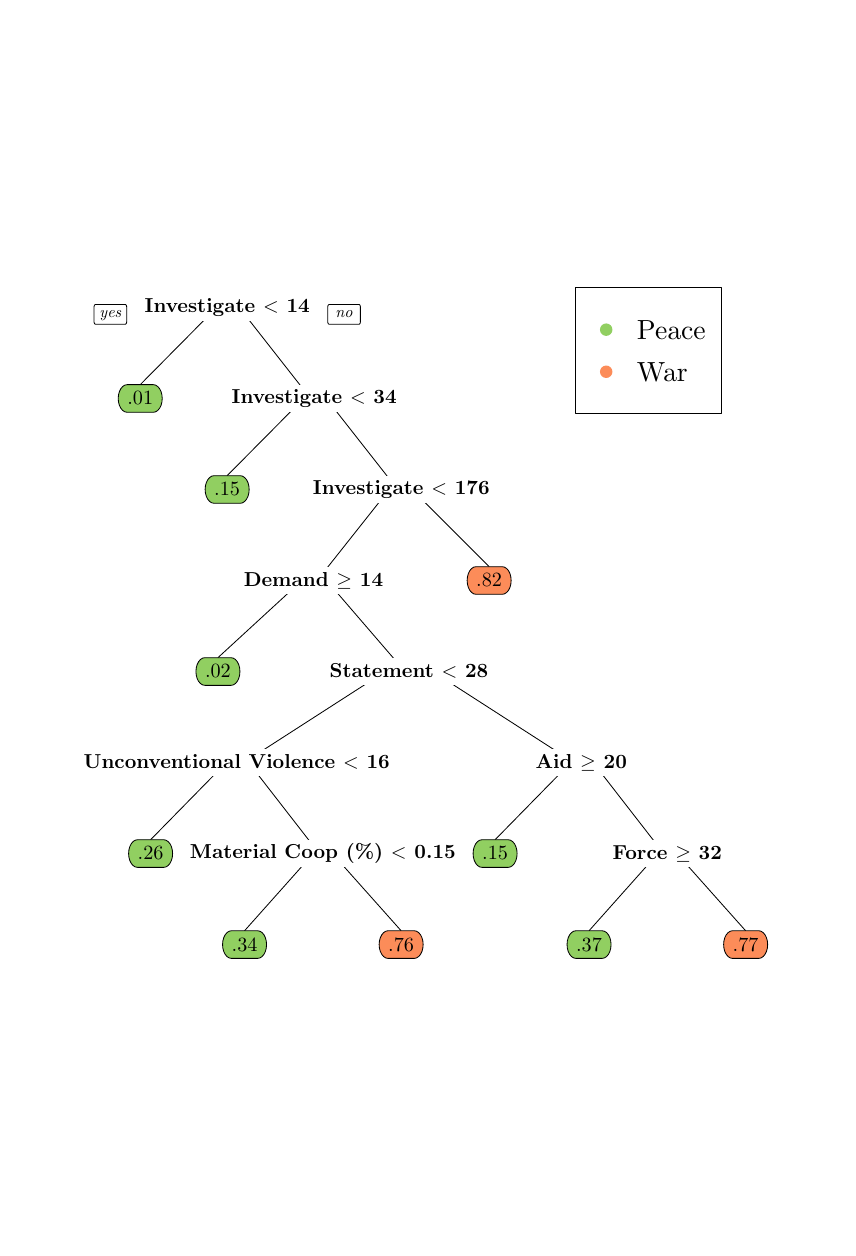
\begin{tikzpicture}[x=1pt,y=1pt]
\definecolor[named]{fillColor}{rgb}{1.00,1.00,1.00}
\path[use as bounding box,fill=fillColor,fill opacity=0.00] (0,0) rectangle (289.08,433.62);
\begin{scope}
\path[clip] (  0.00,  0.00) rectangle (289.08,433.62);
\definecolor[named]{drawColor}{rgb}{0.00,0.00,0.00}

\path[draw=drawColor,line width= 0.3pt,line join=round] ( 40.67,304.62) --
	( 65.82,330.02) --
	( 72.11,330.02);

\path[draw=drawColor,line width= 0.3pt,line join=round] (103.54,297.96) --
	( 78.39,330.02) --
	( 72.11,330.02);

\path[draw=drawColor,line width= 0.3pt,line join=round] ( 72.08,271.73) --
	( 97.25,297.13) --
	(103.54,297.13);

\path[draw=drawColor,line width= 0.3pt,line join=round] (135.01,265.07) --
	(109.84,297.13) --
	(103.54,297.13);

\path[draw=drawColor,line width= 0.3pt,line join=round] (103.27,232.19) --
	(128.66,264.24) --
	(135.01,264.24);

\path[draw=drawColor,line width= 0.3pt,line join=round] ( 68.75,205.96) --
	( 96.36,231.35) --
	(103.27,231.35);

\path[draw=drawColor,line width= 0.3pt,line join=round] (137.78,199.30) --
	(110.17,231.35) --
	(103.27,231.35);

\path[draw=drawColor,line width= 0.3pt,line join=round] ( 75.54,166.41) --
	(125.33,198.47) --
	(137.78,198.47);

\path[draw=drawColor,line width= 0.3pt,line join=round] ( 44.42,140.18) --
	( 69.32,165.58) --
	( 75.54,165.58);

\path[draw=drawColor,line width= 0.3pt,line join=round] (106.66,133.52) --
	( 81.76,165.58) --
	( 75.54,165.58);

\path[draw=drawColor,line width= 0.3pt,line join=round] ( 78.37,107.29) --
	(101.00,132.69) --
	(106.66,132.69);

\path[draw=drawColor,line width= 0.3pt,line join=round] (134.95,107.29) --
	(112.32,132.69) --
	(106.66,132.69);

\path[draw=drawColor,line width= 0.3pt,line join=round] (200.02,166.41) --
	(150.23,198.47) --
	(137.78,198.47);

\path[draw=drawColor,line width= 0.3pt,line join=round] (168.90,140.18) --
	(193.80,165.58) --
	(200.02,165.58);

\path[draw=drawColor,line width= 0.3pt,line join=round] (231.14,133.52) --
	(206.25,165.58) --
	(200.02,165.58);

\path[draw=drawColor,line width= 0.3pt,line join=round] (202.85,107.29) --
	(225.48,132.69) --
	(231.14,132.69);

\path[draw=drawColor,line width= 0.3pt,line join=round] (259.43,107.29) --
	(236.80,132.69) --
	(231.14,132.69);

\path[draw=drawColor,line width= 0.3pt,line join=round] (166.75,238.84) --
	(141.36,264.24) --
	(135.01,264.24);
\definecolor[named]{fillColor}{rgb}{1.00,1.00,1.00}

\path[fill=fillColor] ( 38.12,327.52) --
	( 38.12,337.52) --
	(106.09,337.52) --
	(106.09,327.52) --
	( 38.12,327.52) --
	cycle;

\path[fill=fillColor] ( 69.56,294.63) --
	( 69.56,304.64) --
	(137.52,304.64) --
	(137.52,294.63) --
	( 69.56,294.63) --
	cycle;

\path[fill=fillColor] ( 98.94,261.74) --
	( 98.94,271.75) --
	(171.07,271.75) --
	(171.07,261.74) --
	( 98.94,261.74) --
	cycle;

\path[fill=fillColor] ( 70.64,228.85) --
	( 70.64,238.86) --
	(135.89,238.86) --
	(135.89,228.85) --
	( 70.64,228.85) --
	cycle;

\path[fill=fillColor] (104.94,195.96) --
	(104.94,205.97) --
	(170.62,205.97) --
	(170.62,195.96) --
	(104.94,195.96) --
	cycle;

\path[fill=fillColor] ( 16.26,163.08) --
	( 16.26,173.08) --
	(134.83,173.08) --
	(134.83,163.08) --
	( 16.26,163.08) --
	cycle;

\path[fill=fillColor] ( 54.60,130.19) --
	( 54.60,140.19) --
	(158.72,140.19) --
	(158.72,130.19) --
	( 54.60,130.19) --
	cycle;

\path[fill=fillColor] (176.01,163.08) --
	(176.01,173.08) --
	(224.03,173.08) --
	(224.03,163.08) --
	(176.01,163.08) --
	cycle;

\path[fill=fillColor] (203.92,130.19) --
	(203.92,140.19) --
	(258.37,140.19) --
	(258.37,130.19) --
	(203.92,130.19) --
	cycle;

\node[text=drawColor,anchor=base,inner sep=0pt, outer sep=0pt, scale=  0.73] at ( 72.11,330.72) {\bfseries Investigate $<$ 14};

\node[text=drawColor,anchor=base,inner sep=0pt, outer sep=0pt, scale=  0.73] at (103.54,297.84) {\bfseries Investigate $<$ 34};

\node[text=drawColor,anchor=base,inner sep=0pt, outer sep=0pt, scale=  0.73] at (135.01,264.95) {\bfseries Investigate $<$ 176};

\node[text=drawColor,anchor=base,inner sep=0pt, outer sep=0pt, scale=  0.73] at (103.27,231.71) {\bfseries Demand $\geq$ 14};

\node[text=drawColor,anchor=base,inner sep=0pt, outer sep=0pt, scale=  0.73] at (137.78,198.82) {\bfseries Statement $<$ 28};

\node[text=drawColor,anchor=base,inner sep=0pt, outer sep=0pt, scale=  0.73] at ( 75.54,165.93) {\bfseries Unconventional Violence $<$ 16};

\node[text=drawColor,anchor=base,inner sep=0pt, outer sep=0pt, scale=  0.73] at (106.66,133.38) {\bfseries Material Coop (\%) $<$ 0.15};

\node[text=drawColor,anchor=base,inner sep=0pt, outer sep=0pt, scale=  0.73] at (200.02,165.93) {\bfseries Aid $\geq$ 20};

\node[text=drawColor,anchor=base,inner sep=0pt, outer sep=0pt, scale=  0.73] at (231.14,133.04) {\bfseries Force $\geq$ 32};
\definecolor[named]{fillColor}{rgb}{0.57,0.81,0.38}

\path[draw=drawColor,line width= 0.3pt,line join=round,line cap=round,fill=fillColor] ( 32.71,299.63) --
	( 32.82,300.92) --
	( 33.15,302.12) --
	( 33.66,303.16) --
	( 34.33,303.95) --
	( 35.11,304.45) --
	( 35.95,304.62) --
	( 45.39,304.62) --
	( 46.23,304.45) --
	( 47.00,303.95) --
	( 47.67,303.16) --
	( 48.19,302.12) --
	( 48.51,300.92) --
	( 48.62,299.63) --
	( 48.62,299.63) --
	( 48.51,298.34) --
	( 48.19,297.13) --
	( 47.67,296.10) --
	( 47.00,295.30) --
	( 46.23,294.80) --
	( 45.39,294.63) --
	( 35.95,294.63) --
	( 35.11,294.80) --
	( 34.33,295.30) --
	( 33.66,296.10) --
	( 33.15,297.13) --
	( 32.82,298.34) --
	( 32.71,299.63) --
	cycle;

\path[draw=drawColor,line width= 0.3pt,line join=round,line cap=round,fill=fillColor] ( 64.12,266.74) --
	( 64.23,268.03) --
	( 64.56,269.24) --
	( 65.07,270.27) --
	( 65.74,271.06) --
	( 66.52,271.56) --
	( 67.36,271.73) --
	( 76.80,271.73) --
	( 77.64,271.56) --
	( 78.41,271.06) --
	( 79.08,270.27) --
	( 79.60,269.24) --
	( 79.92,268.03) --
	( 80.03,266.74) --
	( 80.03,266.74) --
	( 79.92,265.45) --
	( 79.60,264.24) --
	( 79.08,263.21) --
	( 78.41,262.42) --
	( 77.64,261.92) --
	( 76.80,261.75) --
	( 67.36,261.75) --
	( 66.52,261.92) --
	( 65.74,262.42) --
	( 65.07,263.21) --
	( 64.56,264.24) --
	( 64.23,265.45) --
	( 64.12,266.74) --
	cycle;

\path[draw=drawColor,line width= 0.3pt,line join=round,line cap=round,fill=fillColor] ( 60.80,200.96) --
	( 60.91,202.26) --
	( 61.23,203.46) --
	( 61.74,204.49) --
	( 62.41,205.29) --
	( 63.19,205.79) --
	( 64.03,205.96) --
	( 73.47,205.96) --
	( 74.31,205.79) --
	( 75.09,205.29) --
	( 75.76,204.49) --
	( 76.27,203.46) --
	( 76.59,202.26) --
	( 76.70,200.96) --
	( 76.70,200.96) --
	( 76.59,199.67) --
	( 76.27,198.47) --
	( 75.76,197.43) --
	( 75.09,196.64) --
	( 74.31,196.14) --
	( 73.47,195.97) --
	( 64.03,195.97) --
	( 63.19,196.14) --
	( 62.41,196.64) --
	( 61.74,197.43) --
	( 61.23,198.47) --
	( 60.91,199.67) --
	( 60.80,200.96) --
	cycle;

\path[draw=drawColor,line width= 0.3pt,line join=round,line cap=round,fill=fillColor] ( 36.47,135.19) --
	( 36.58,136.48) --
	( 36.90,137.68) --
	( 37.41,138.72) --
	( 38.08,139.51) --
	( 38.86,140.01) --
	( 39.70,140.18) --
	( 49.14,140.18) --
	( 49.98,140.01) --
	( 50.76,139.51) --
	( 51.43,138.72) --
	( 51.94,137.68) --
	( 52.26,136.48) --
	( 52.37,135.19) --
	( 52.37,135.19) --
	( 52.26,133.89) --
	( 51.94,132.69) --
	( 51.43,131.66) --
	( 50.76,130.86) --
	( 49.98,130.36) --
	( 49.14,130.19) --
	( 39.70,130.19) --
	( 38.86,130.36) --
	( 38.08,130.86) --
	( 37.41,131.66) --
	( 36.90,132.69) --
	( 36.58,133.89) --
	( 36.47,135.19) --
	cycle;

\path[draw=drawColor,line width= 0.3pt,line join=round,line cap=round,fill=fillColor] ( 70.42,102.30) --
	( 70.53,103.59) --
	( 70.85,104.79) --
	( 71.36,105.83) --
	( 72.03,106.62) --
	( 72.81,107.12) --
	( 73.65,107.29) --
	( 83.09,107.29) --
	( 83.93,107.12) --
	( 84.71,106.62) --
	( 85.38,105.83) --
	( 85.89,104.79) --
	( 86.21,103.59) --
	( 86.32,102.30) --
	( 86.32,102.30) --
	( 86.21,101.01) --
	( 85.89, 99.80) --
	( 85.38, 98.77) --
	( 84.71, 97.97) --
	( 83.93, 97.47) --
	( 83.09, 97.30) --
	( 73.65, 97.30) --
	( 72.81, 97.47) --
	( 72.03, 97.97) --
	( 71.36, 98.77) --
	( 70.85, 99.80) --
	( 70.53,101.01) --
	( 70.42,102.30) --
	cycle;
\definecolor[named]{fillColor}{rgb}{0.99,0.55,0.35}

\path[draw=drawColor,line width= 0.3pt,line join=round,line cap=round,fill=fillColor] (127.00,102.30) --
	(127.11,103.59) --
	(127.43,104.79) --
	(127.95,105.83) --
	(128.61,106.62) --
	(129.39,107.12) --
	(130.23,107.29) --
	(139.67,107.29) --
	(140.51,107.12) --
	(141.29,106.62) --
	(141.96,105.83) --
	(142.47,104.79) --
	(142.79,103.59) --
	(142.90,102.30) --
	(142.90,102.30) --
	(142.79,101.01) --
	(142.47, 99.80) --
	(141.96, 98.77) --
	(141.29, 97.97) --
	(140.51, 97.47) --
	(139.67, 97.30) --
	(130.23, 97.30) --
	(129.39, 97.47) --
	(128.61, 97.97) --
	(127.95, 98.77) --
	(127.43, 99.80) --
	(127.11,101.01) --
	(127.00,102.30) --
	cycle;
\definecolor[named]{fillColor}{rgb}{0.57,0.81,0.38}

\path[draw=drawColor,line width= 0.3pt,line join=round,line cap=round,fill=fillColor] (160.95,135.19) --
	(161.06,136.48) --
	(161.38,137.68) --
	(161.89,138.72) --
	(162.56,139.51) --
	(163.34,140.01) --
	(164.18,140.18) --
	(173.62,140.18) --
	(174.46,140.01) --
	(175.24,139.51) --
	(175.91,138.72) --
	(176.42,137.68) --
	(176.74,136.48) --
	(176.85,135.19) --
	(176.85,135.19) --
	(176.74,133.89) --
	(176.42,132.69) --
	(175.91,131.66) --
	(175.24,130.86) --
	(174.46,130.36) --
	(173.62,130.19) --
	(164.18,130.19) --
	(163.34,130.36) --
	(162.56,130.86) --
	(161.89,131.66) --
	(161.38,132.69) --
	(161.06,133.89) --
	(160.95,135.19) --
	cycle;

\path[draw=drawColor,line width= 0.3pt,line join=round,line cap=round,fill=fillColor] (194.90,102.30) --
	(195.01,103.59) --
	(195.33,104.79) --
	(195.84,105.83) --
	(196.51,106.62) --
	(197.29,107.12) --
	(198.13,107.29) --
	(207.57,107.29) --
	(208.41,107.12) --
	(209.19,106.62) --
	(209.86,105.83) --
	(210.37,104.79) --
	(210.69,103.59) --
	(210.80,102.30) --
	(210.80,102.30) --
	(210.69,101.01) --
	(210.37, 99.80) --
	(209.86, 98.77) --
	(209.19, 97.97) --
	(208.41, 97.47) --
	(207.57, 97.30) --
	(198.13, 97.30) --
	(197.29, 97.47) --
	(196.51, 97.97) --
	(195.84, 98.77) --
	(195.33, 99.80) --
	(195.01,101.01) --
	(194.90,102.30) --
	cycle;
\definecolor[named]{fillColor}{rgb}{0.99,0.55,0.35}

\path[draw=drawColor,line width= 0.3pt,line join=round,line cap=round,fill=fillColor] (251.48,102.30) --
	(251.59,103.59) --
	(251.91,104.79) --
	(252.43,105.83) --
	(253.10,106.62) --
	(253.88,107.12) --
	(254.71,107.29) --
	(264.16,107.29) --
	(264.99,107.12) --
	(265.77,106.62) --
	(266.44,105.83) --
	(266.95,104.79) --
	(267.28,103.59) --
	(267.39,102.30) --
	(267.39,102.30) --
	(267.28,101.01) --
	(266.95, 99.80) --
	(266.44, 98.77) --
	(265.77, 97.97) --
	(264.99, 97.47) --
	(264.16, 97.30) --
	(254.71, 97.30) --
	(253.88, 97.47) --
	(253.10, 97.97) --
	(252.43, 98.77) --
	(251.91, 99.80) --
	(251.59,101.01) --
	(251.48,102.30) --
	cycle;

\path[draw=drawColor,line width= 0.3pt,line join=round,line cap=round,fill=fillColor] (158.80,233.85) --
	(158.91,235.14) --
	(159.23,236.35) --
	(159.74,237.38) --
	(160.41,238.18) --
	(161.19,238.67) --
	(162.03,238.84) --
	(171.47,238.84) --
	(172.31,238.67) --
	(173.09,238.18) --
	(173.76,237.38) --
	(174.27,236.35) --
	(174.59,235.14) --
	(174.70,233.85) --
	(174.70,233.85) --
	(174.59,232.56) --
	(174.27,231.35) --
	(173.76,230.32) --
	(173.09,229.53) --
	(172.31,229.03) --
	(171.47,228.86) --
	(162.03,228.86) --
	(161.19,229.03) --
	(160.41,229.53) --
	(159.74,230.32) --
	(159.23,231.35) --
	(158.91,232.56) --
	(158.80,233.85) --
	cycle;

\node[text=drawColor,anchor=base,inner sep=0pt, outer sep=0pt, scale=  0.73] at ( 40.67,297.30) {.01};

\node[text=drawColor,anchor=base,inner sep=0pt, outer sep=0pt, scale=  0.73] at ( 72.08,264.41) {.15};

\node[text=drawColor,anchor=base,inner sep=0pt, outer sep=0pt, scale=  0.73] at ( 68.75,198.64) {.02};

\node[text=drawColor,anchor=base,inner sep=0pt, outer sep=0pt, scale=  0.73] at ( 44.42,132.86) {.26};

\node[text=drawColor,anchor=base,inner sep=0pt, outer sep=0pt, scale=  0.73] at ( 78.37, 99.97) {.34};

\node[text=drawColor,anchor=base,inner sep=0pt, outer sep=0pt, scale=  0.73] at (134.95, 99.97) {.76};

\node[text=drawColor,anchor=base,inner sep=0pt, outer sep=0pt, scale=  0.73] at (168.90,132.86) {.15};

\node[text=drawColor,anchor=base,inner sep=0pt, outer sep=0pt, scale=  0.73] at (202.85, 99.97) {.37};

\node[text=drawColor,anchor=base,inner sep=0pt, outer sep=0pt, scale=  0.73] at (259.43, 99.97) {.77};

\node[text=drawColor,anchor=base,inner sep=0pt, outer sep=0pt, scale=  0.73] at (166.75,231.53) {.82};
\definecolor[named]{fillColor}{rgb}{1.00,1.00,1.00}

\path[draw=drawColor,line width= 0.3pt,line join=round,line cap=round,fill=fillColor] ( 23.99,332.72) --
	( 24.01,332.95) --
	( 24.06,333.17) --
	( 24.16,333.35) --
	( 24.28,333.49) --
	( 24.42,333.58) --
	( 24.57,333.61) --
	( 35.19,333.61) --
	( 35.34,333.58) --
	( 35.48,333.49) --
	( 35.60,333.35) --
	( 35.69,333.17) --
	( 35.75,332.95) --
	( 35.77,332.72) --
	( 35.77,327.32) --
	( 35.75,327.09) --
	( 35.69,326.87) --
	( 35.60,326.69) --
	( 35.48,326.54) --
	( 35.34,326.46) --
	( 35.19,326.42) --
	( 24.57,326.42) --
	( 24.42,326.46) --
	( 24.28,326.54) --
	( 24.16,326.69) --
	( 24.06,326.87) --
	( 24.01,327.09) --
	( 23.99,327.32) --
	cycle;

\path[draw=drawColor,line width= 0.3pt,line join=round,line cap=round,fill=fillColor] (108.44,332.72) --
	(108.46,332.95) --
	(108.52,333.17) --
	(108.61,333.35) --
	(108.73,333.49) --
	(108.87,333.58) --
	(109.02,333.61) --
	(119.64,333.61) --
	(119.79,333.58) --
	(119.93,333.49) --
	(120.05,333.35) --
	(120.15,333.17) --
	(120.20,332.95) --
	(120.22,332.72) --
	(120.22,327.32) --
	(120.20,327.09) --
	(120.15,326.87) --
	(120.05,326.69) --
	(119.93,326.54) --
	(119.79,326.46) --
	(119.64,326.42) --
	(109.02,326.42) --
	(108.87,326.46) --
	(108.73,326.54) --
	(108.61,326.69) --
	(108.52,326.87) --
	(108.46,327.09) --
	(108.44,327.32) --
	cycle;

\node[text=drawColor,anchor=base,inner sep=0pt, outer sep=0pt, scale=  0.58] at ( 29.88,328.74) {\itshape yes};

\node[text=drawColor,anchor=base,inner sep=0pt, outer sep=0pt, scale=  0.58] at (114.33,328.77) {\itshape no};
\end{scope}
\begin{scope}
\path[clip] ( 49.20, 61.20) rectangle (263.88,384.42);
\definecolor[named]{drawColor}{rgb}{0.00,0.00,0.00}

\path[draw=drawColor,line width= 0.4pt,line join=round,line cap=round] (197.93,339.70) rectangle (250.57,294.07);
\definecolor[named]{fillColor}{rgb}{0.57,0.81,0.38}

\path[fill=fillColor] (209.05,324.49) circle (  2.25);
\definecolor[named]{fillColor}{rgb}{0.99,0.55,0.35}

\path[fill=fillColor] (209.05,309.28) circle (  2.25);

\node[text=drawColor,anchor=base west,inner sep=0pt, outer sep=0pt, scale=  1.00] at (220.16,321.04) {Peace};

\node[text=drawColor,anchor=base west,inner sep=0pt, outer sep=0pt, scale=  1.00] at (220.16,305.84) {War};
\end{scope}
\end{tikzpicture}

    \caption{Fitted and Pruned Classification Tree}
    \label{tree}
  \end{center}
\end{figure}

\subsection{Interpretation}

To interpret the tree, we begin at the top (root) node and work downward. The inequality at listed at each node splits the data. If the observation satisfies the inequality, we visit the left subtree; otherwise, we visit the right subtree. We continue recursively until we reach a leaf, which indicates whether that dyad month should be classified as peaceful (green) or at war (red). For example, an observation with less than 14 investigations in that dyad-month would cause us to trace the left subtree of the root note, and classify that observation as peaceful (war occurs in less than one percent of such observations). By contrast, a month with between 34 and 176 investigations, more than 28 statements, and at least 32 acts of force has about a 77 percent chance of being at war in the training data. 

All of the twenty event types described above were supplied as candidate variables to the model, as were the percentage of observations within each quadrant (i.e. material cooperation, verbal cooperation, material conflict, and verbal conflict). Of these, seven variables are included in the final tree. Investigations feature prominently in the first three splits. At first this seemed curious, given that investigations are classified as material cooperation by CAMEO (compare node eight). Upon closer examination, this category includes investigations of crime, corruption, human rights abuses, military action, and war crimes. Given that humanitarian interventions feature prominently in the MID dataset during the period under consideration, the influence of this variable becomes less surprising. For example, NATO efforts in the Balkans involve a large number of dyads involved in the investigation of war crimes and other human rights violations. 

The other splits are less surprising. Demands (node four) are likely to be more associated with domestic conflicts, such as protest movements, rather than interstate disputes. Large amounts of aid make conflict less likely (node seven), as would be expected. Unconventional violence (e.g. mass killings and ethnic cleansing) and the use of force (e.g. fighting with small arms, artillery, or aircraft) are associated with MIDs for obvious reasons. Overall the model seems to match the types of conflict observed in the 1990s, but might do less well in later periods. 

\subsection{Model Diagnostics}

How does the tree perform relative to other classification models? Table \ref{cart-perf} compares the tree above to a null model (all observations are predicted to be peaceful) and a logistic regression using the same features as the CART model. The data was split into two parts, a training set for fitting the models, and a test set for out-of-sample comparison. This prevents a model that overfits the data from appearing superior to one with more generality. 

Mean-squared error is the average squared deviation of predictions from the observed values. It is calculated as $MSE=\frac{1}{n}\sum_{i=1}^n (y_i - \hat{y}_i)^2$. The ideal MSE is zero, and in this case the worst possible value is 1. In the case of binary classification, this is equal to the misclassification rate. Precision and recall are particularly useful metrics for rare events, as they penalize the model for making incorrect prediction. The ideal for both is a value of 1. Precision is calculated as the proportion of true positives relative to the number of true and false positives (i.e. $\# \text{accurate predictions of war} \over \text{\# total predictions of war}$). Recall is similar, but for the proportion of true positives relative to the number of true positives and false negatives (i.e. $\# \text{accurate predictions of war} \over \text{\# total observed cases of war}$).

The classification tree outperforms the other two models in the training data (1992-1998, $n=372,271$). For the test data (1999-2001, $n=213,218$), the tree has the same mean-squared error (MSE) as the null model, but better precision and recall. Compared to logistic regression, the tree has worse recall but much better precision for the test data. This suggests that the classification tree generated more false negatives (i.e. missed the occurrence of some conflicts) in the test data.

\begin{table}
	\caption{Comparison of CART to Alternative Models}
	\label{cart-perf}
  \begin{center}
  \begin{tabular}{l|ccc|ccc}
   \multicolumn{1}{c}{} & \multicolumn{3}{c}{Training Data} & \multicolumn{3}{c}{Test Data} \\
  Model & MSE & Precision & Recall & MSE & Precision & Recall \\
  \midrule
  Null & 0.0075 & 0.000 & 0.000 & 0.0066 & 0.000 & 0.000 \\
  GLM & 0.0082 & 0.158 & 0.022  & 0.0079 & 0.142 & 0.038 \\
  CART & 0.0067 & 0.702 & 0.192 & 0.0066 & 0.422 & 0.027 
  \end{tabular}
  \end{center}
\end{table}


\section{Conclusion}
\label{conclusion}

Classification trees strike a nice balance between computational and statistical efficiency. The computational complexity of greedy tree-building is $\Theta(n \log n)$, which is the best that can be hoped for. Statistically, CART outperforms logisitic regression using a generalized linear model (GLM). In the application here, this is likely because the classification tree handled dependencies between features better than the linear model. 

The interpretation of the tree suggests that it fits the 1990s very well, but may perform less well in the future. Perhaps an ensemble of trees based on a few months of data at a time (with the addition of more trees as the data extend in to the future) would perform better and account for changes in the data generating process over time. A Bayesian ensemble of several classification trees could improve performance while still maintaining more interpretability than is available in random forests \citep{arva2013improving,montgomery2012improving,Raftery:1995,raftery2005using}.

Other adjustments can also help to refine the model at later stages. International conflict is a relatively rare event, meaning that in $k$-fold cross validation it is possible that some subsets will have no instances of conflict; to prevent this, synthetic minority over-sampling (SMOTE) could be used \citep{chawla2002smote}. To incorporate interdependencies not captured at the dyadic level, future iterations could also include lags that measure conflict in social or spatial neighbors \citep{gleditsch2000war,gleditsch2001measuring,hoff2004modeling,ward1998democratizing,ward2007disputes,ward2011network}.

The findings thus far indicate that automated production of political indicators is feasible to within a close approximation. The application of classification trees offers a quick and inexpensive tool that can save much human effort. A final pass by human coders will still be required to obtain fully accurate classifications, but the cost can be substantially reduced. With the additional steps proposed above, the process of automating political indicators using event data could also be applied to other widely used indices such as the Polity and Freedom House regime scales (measuring democracy and autocracy).



% \renewcommand{\bibsection}{\paragraph{References}}
\pagebreak
\singlespacing
\setlength{\bibsep}{0.0pt}
\bibliographystyle{/Users/mcdickenson/Documents/Templates/chicago}
\bibliography{/Users/mcdickenson/Documents/Templates/RefLib.bib}


\end{document}
